\articlepart{高速化のための配列習得}{tomoemon}

\section{はじめに}

「より速く入力できるようになりたい」というのは競技タイピングに取り組む人なら誰しも思うことです。速く打つための方法論や練習法については本書の他の記事にも載っていますが、この記事では「最初に覚えたキーボード配列とは別の配列」を習得して高速なタイピングを目指す方法について紹介しながら、この方法の良い点、悪い点を考えていきます。

ここでいう「最初に覚えたキーボード配列とは別の配列」とは、例えばローマ字入力を最初に覚えた人にとってのかな入力や、かな入力を最初に覚えた人にとってのローマ字入力が当てはまります。もちろんこれ以外にも、Qwerty配列からDvorak配列に乗り換える、親指シフト配列に乗り換えるといった様々な場合が考えられます。どのようなパターンにせよ、現状の配列に何らかの限界を感じて、それ以外の配列に可能性を感じたときに乗り換えることが多いと思います。ここでは特に入力速度の限界、可能性という観点でこの方法の有効性について考えていきます。

\section{用語の確認}

\subsection{キーボード配列}

「キーボード配列(あるいは単に配列)」という言葉の意味で混乱することがあるので先に説明しておきます。一般的にキーボード配列というとキーボードに印字されている\key{Q}\key{W}\key{E}\key{R}\key{T}\key{Y}という並びのことをイメージすると思いますが、大体それで問題ありません。例えば図\ref{qwerty}はQwerty配列と呼ばれるもので現在広く普及しているものです。


\begin{figure*}
 \begin{center}
   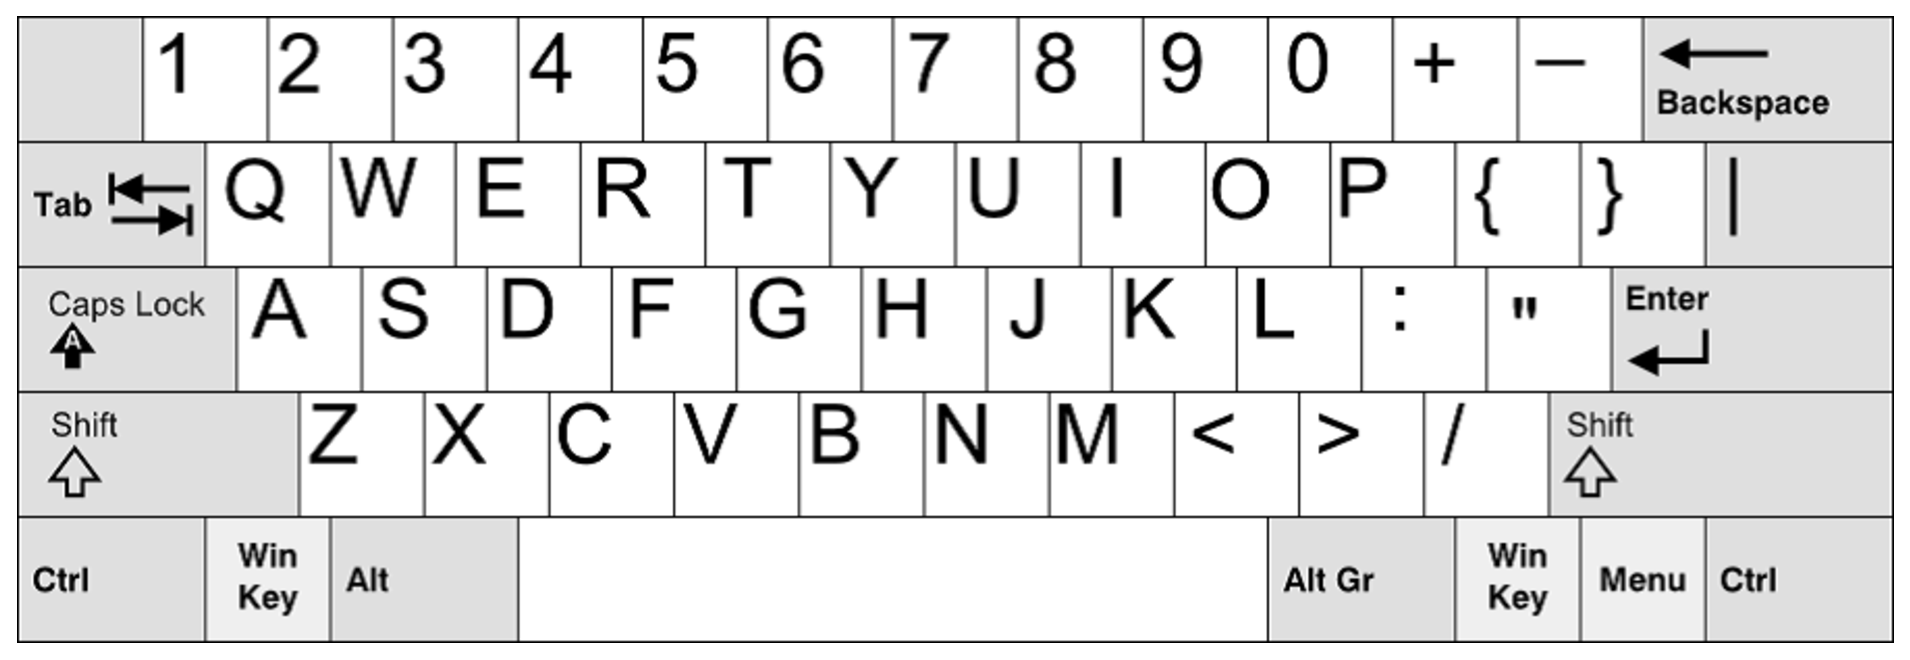
\includegraphics[width=14cm,clip]{res_tomoemon/qwerty.eps}
 \end{center}
 \caption{Qwerty配列}
 \label{qwerty}
\end{figure*}

この配列を使って英字入力モードで\key{Q}を押すと[q]という文字がコンピュータに入力されます。どのキーを押したときに何の文字が入力されるか、という組み合わせをキーボードの論理配列と言い、この記事で配列と言った場合はこれを指します。一方、物理的なキーの形状や位置をキーボードの物理配列と言います。現在のキーボードの多くは各段のキーの位置が少しずつ横にずれていますが、きれいな格子状になっている物理配列のキーボードも存在します。

物理配列と論理配列のイメージがわきにくい方は無刻印モデルキーボード\footnote{\url{http://www.pfu.fujitsu.com/hhkeyboard/hhkbpro2/nokeytop.html}}をイメージすると良いでしょう。

\begin{figure*}
 \begin{center}
   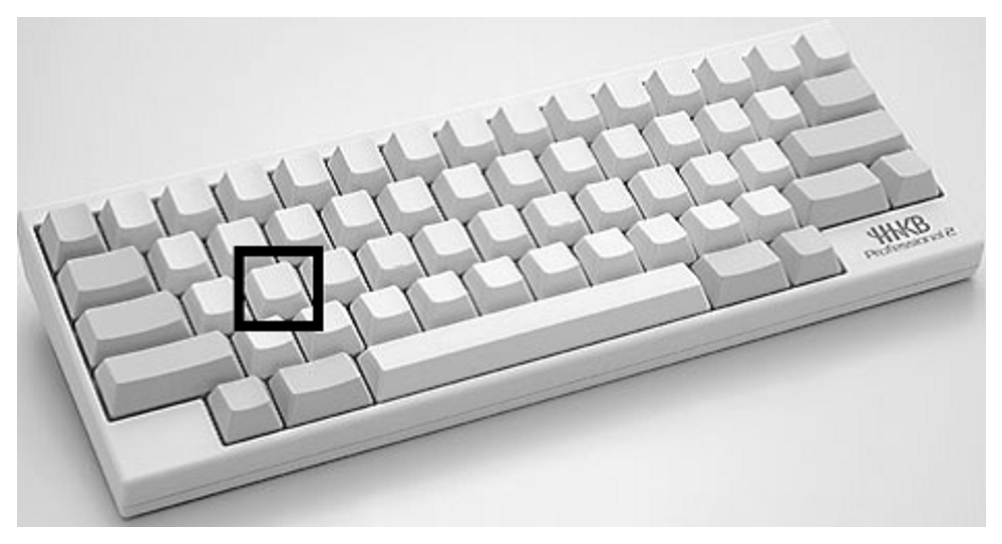
\includegraphics[width=14cm,clip]{res_tomoemon/nokeytop.eps}
 \end{center}
 \caption{Happy Hacking Keyboard Professional2 白/無刻印}
 \label{nokeytop}
\end{figure*}


図\ref{nokeytop}で四角い枠で囲んだ位置のキーを押したときに何の文字が出るかは論理配列によって決まります。Qwerty配列を使っていれば[s]が出ますし、図\ref{dvorak}のDvorak配列では[o]の文字が出ます。

\begin{figure*}
 \begin{center}
   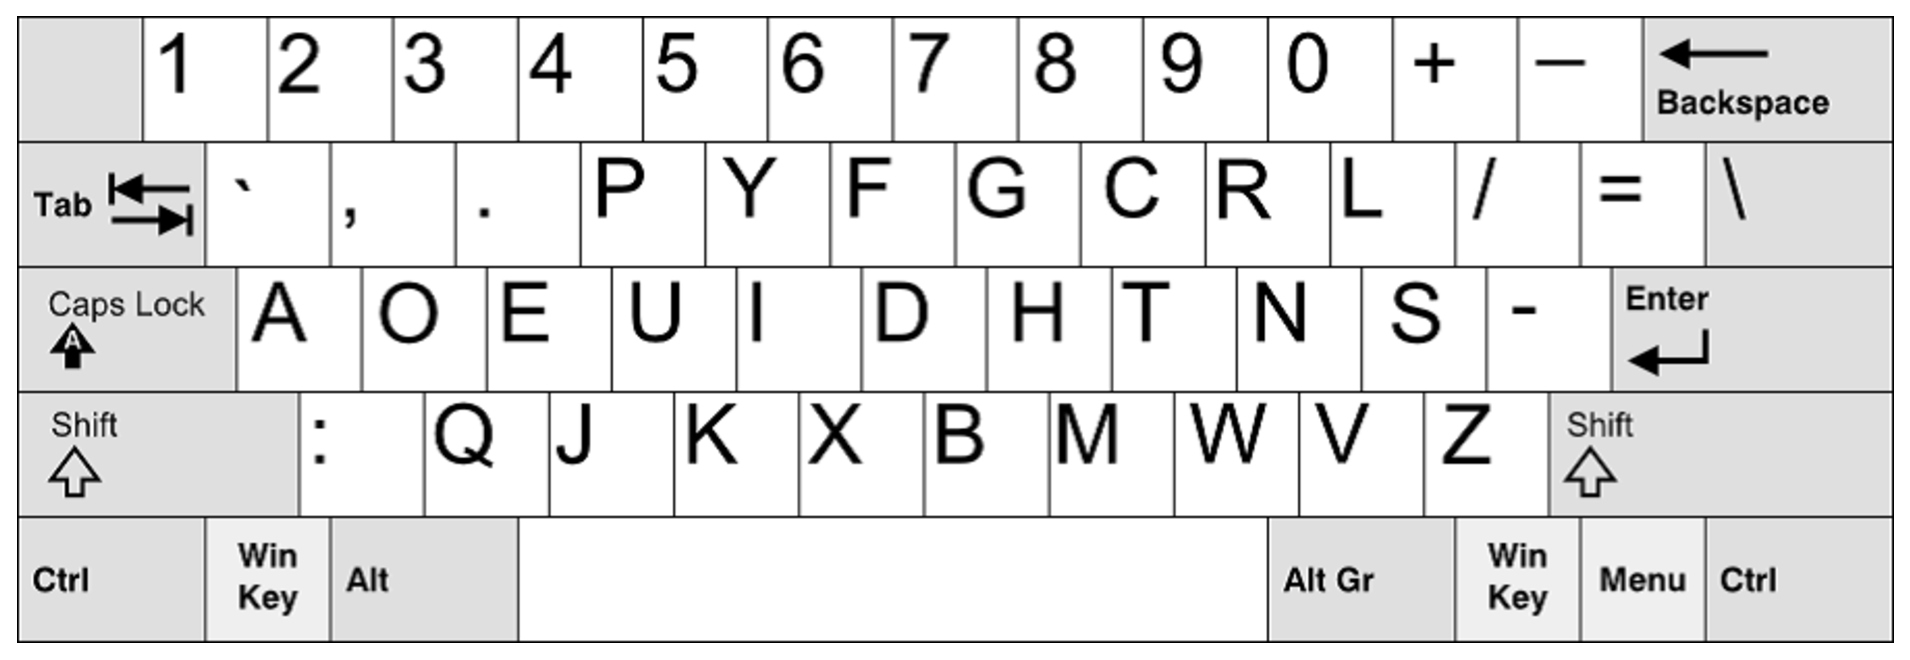
\includegraphics[width=14cm,clip]{res_tomoemon/dvorak.eps}
 \end{center}
 \caption{Dvorak配列}
 \label{dvorak}
\end{figure*}

物理配列の上にはいくつも論理配列を重ねることができ、例えば物理的なキーボード1枚で、Qwertyの英字入力、かな入力、ローマ字入力といった複数の配列を切り替え、または組み合わせて実現することができます。図\ref{arrangement}は物理配列と論理配列の関係を表したものです。

\begin{figure*}
 \begin{center}
   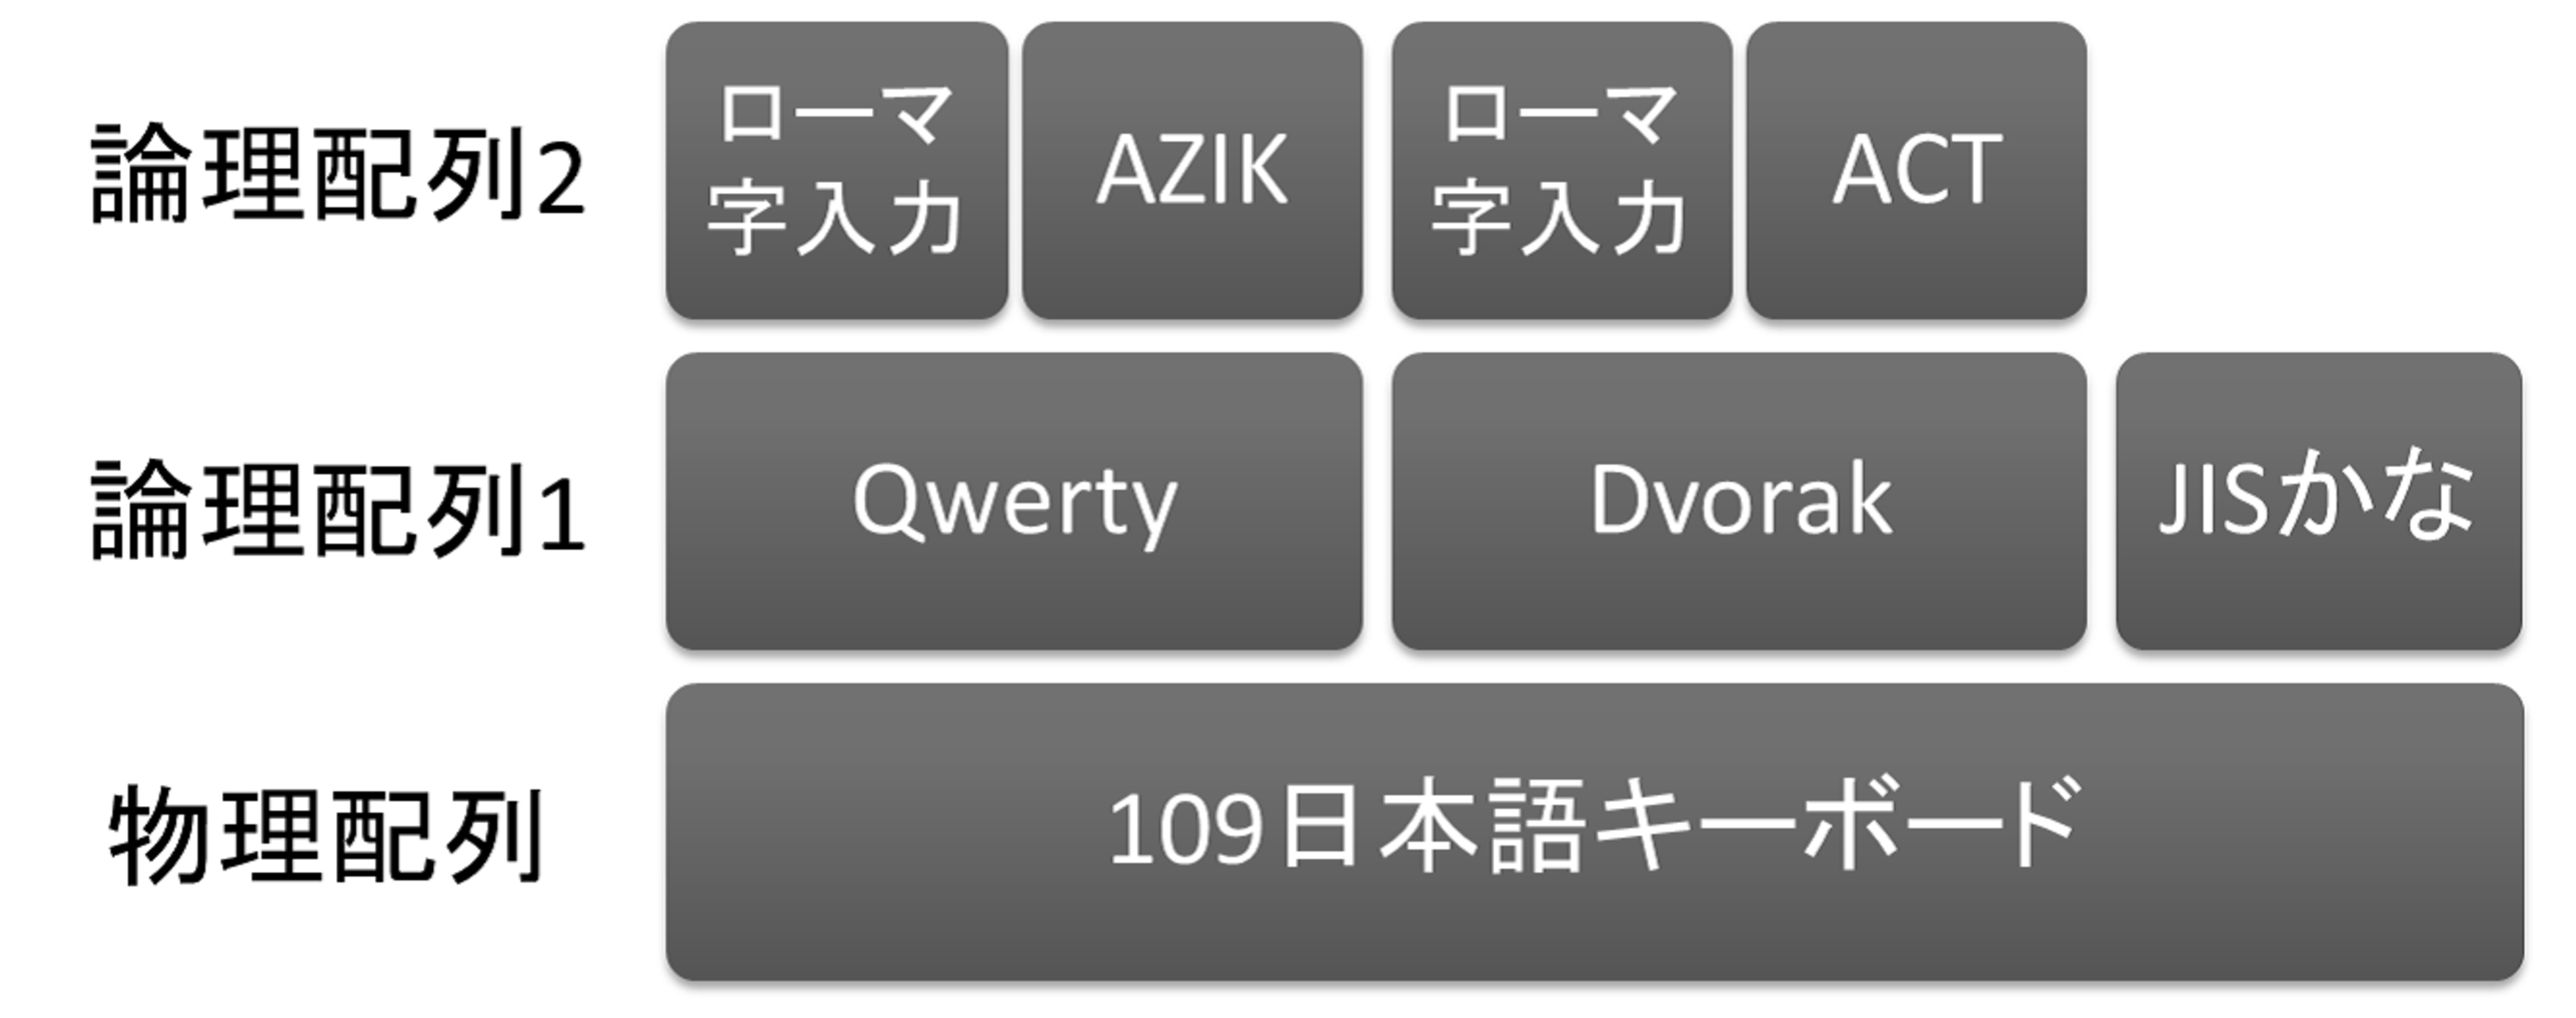
\includegraphics[width=14cm,clip]{res_tomoemon/arrangement.eps}
 \end{center}
 \caption{物理配列と論理配列の階層}
 \label{arrangement}
\end{figure*}

論理配列をざっくりと分けると、英字を入力する配列とかなを入力する配列の二種類に分けることができます\footnote{漢字を直接できる配列もありますがここでは割愛します。}。ローマ字入力も最終的にはかなを入力する配列なので、ここではかな入力の一つとします。ただし、ローマ字入力は英字の組み合わせで入力するため、図\ref{arrangement}のように英字入力の配列に依存しています。

\subsection{入力速度と打鍵速度}

これは特に難しいことはないのですが、「入力速度」「速い」「遅い」という言葉をよく使うので、それぞれの意味を確認しておきます。まず、入力速度を、[課題の文字数]÷[入力に要した時間]と定義します。競技タイピングにおいて、入力すべき文字はすべて与えられているので、これを課題の文字列と呼び、その文字数を「課題の文字数」とします。ここでは英字、かな、かな漢字混じりなどは気にしません。また、入力可能な状態になってから入力が完了するまでの時間を「入力に要した時間」とします。具体例で説明すると「こんにちは」を4秒で打ち切った場合の入力速度は1.25文字/秒です。入力速度が「速い」とはこの入力速度の値が大きいこと、「遅い」はその逆を表します。
これとは別に「打鍵速度」という言い方をする場合があります。これは単純で、単位時間あたりにキーボードのキーを何回打鍵できるかを表すものです。一般的に高速に打鍵できる方が高速な入力になりますが、変換ありの日本語入力速度を競う場合は変換に卓越した人が打鍵速度で劣っていても入力速度で勝る場合が十分にありえます。

\section{なぜ配列を変えるのか}

さて、ようやく本題ですが、そもそもなぜ配列を変えなければいけないのでしょうか。マイナー配列を好んで使おうとするタイパーがいるのはなぜでしょうか。後述する通り配列を変えるというのは大きな労力を必要としますが、苦労して配列を変えるからにはそれなりのメリットも存在するのです。

\begin{itemize}
 \item 指の動きに無理がなくなる
 \item 同指打鍵が減る
 \item 同鍵連打が減る
 \item 指の移動距離が減る
 \item 指の移動範囲が狭くなる
 \item 打鍵の回数が減る
 \item 動かしやすい指を重点的に使う
\end{itemize}
これらはどれも高速打鍵にとって重要と考えられる要素で、これらを自在にコントロールできるようになるのが「配列を変える」という手法です。ここが配列を変える動機の肝なので、ローマ字入力を例に少し説明をしておきます。

\subsubsection*{指の動きに無理がなくなる}
「わざわざ」を打つ場合、標準運指では薬指と小指で\finger{21112111}となりますが、これは非常に打ちにくいパターンになります。配列を変えることでこういったパターンを減らし、打ちやすいパターンに変えることができます。
\subsubsection*{同指打鍵が減る}
「ぬくぬく」と打つ場合は\finger{77877787}となって「ぬ」を打つために人差し指が2段分動きますが、このような指の移動は高速化が難しいため、できるだけ少ないほうが好ましいです。
\subsubsection*{同鍵連打が減る}
「なんの」と打つ場合「nannno」となり、\key{N}を3回連続で打つ必要がありますが、同じキーを連続で打つのも遅くなる要因になります。この場合は「naxnno」と打って1回分減らすことができますが、小さい「つ」が入る場合は避けることができません。
\subsubsection*{指の移動距離が減る}
指を移動しないで打つことができれば当然速くなります\footnote{同じ指で同じキーを連打する場合は例外的に遅くなることがあります。}。配列によってはホームポジションからほとんど指を動かさずに打てることをメリットとしてあげているものもあります。
\subsubsection*{指の移動範囲が狭くなる}
上記に近い要素で、かな入力の場合は4段使うのに対し、ローマ字入力では3段しか使わないといった配列ごとの違いがあります。広い範囲を使う方が1打鍵で入力できる文字の種類が増えて高速化できる一方、指の移動範囲が広くなることでミスの少ない安定した入力が難しくなるという一長一短があります。
\subsubsection*{打鍵の回数が減る}
より少ない打鍵回数で同じ文字列を打てるようにすることができます。ローマ字入力の「こんにちは」は10打鍵ですが、かな入力では5打鍵になります。
\subsubsection*{動かしやすい指を重点的に使う}
右利きの人は当然右手の方が動かしやすく、また利き手に関わらず人差し指や中指が動かしやすいことと思います。配列と入力する文章の組み合わせによってはそれ以外の指を多く使うといったことが起こりえます。この場合、苦手な指を練習によって鍛えるのもありですが、動かしやすい指を重点的に使う配列を使うことで、全体から見てより高速に打てるようになります。

これらの特徴を踏まえ、各人にとって適切な配列に切り替えることで「入力速度が速く」なります。ただし、例の中でも説明している通り、これらは必ずしも配列を変更することでしか得られないメリットではなく、我流運指を取り入れる等の「最適化」テクニックによってカバーできる範囲も多々あります。しかし、例えば最適化では打鍵回数を減らすことはできません。最適化よりも柔軟に、かつ自由に上記要素を改善できるのが配列を変えるという手法になります。配列ごとに特にどの要素を重視しているか異なるため、配列を選択する際は自分が重視したい要素とのマッチングが重要になります。

私の場合はAZIKという配列をベースにしたものを使っています。この配列ではローマ字入力で割り当てられていない英字の組み合わせに別のかなを割り当てて、元のローマ字入力はほぼ維持しつつ、より少ない打鍵の打ちやすいパターンを増やしています。例えば表\ref{tomoemon:compare_roman_azik}のような打ち方ができます。

\begin{table}
\begin{center}
\caption{ローマ字入力とAZIKの比較}
\label{tomoemon:compare_roman_azik}
\begin{tabular}{ccc}
\hline
かな & ローマ字入力 & AZIK \\
\hline
かん きん こん & kan kin kon & kn kk kl \\
しゃ しゅ しょ & sha shu sho & xa xu xo \\
にゃ にゅ にょ & nya nyu nyo & nga ngu ngo \\
がっこう & gakkou & ga;kp \\
\hline
\end{tabular}
\end{center}
\end{table}

元のローマ字入力の大部分がそのまま使えるという特徴から、通常のローマ字入力を使いつつ徐々に効率的な打ち方をしていくことができるというメリットを持ちますが、それゆえに劇的な変化は望めないということになります。何をメリットと感じ何をデメリットと感じるかは、人それぞれなので、自分の目指すものと配列ごとの特徴をよく知ることが重要です。

\section{配列を変更すべきでない5つの理由}

メリットだけ説明してあとは自己責任でというのも不親切なので、配列変更すべきでない理由も合わせて説明しておきます。実際のところメリットについてはいろいろなところで紹介されているので、重要になるのはデメリットの方だったりします。いろんな配列にチャレンジして欲しい立場としては携帯電話の料金プランのことわり書きのように極小フォントで書きたいところですが、デメリットも理解した上でのチャレンジをお勧めします。さて、先述のようなメリットを享受するために支払うコストとリスクは小さくありません。異なる配列を習得するためにあなたは少なくとも次の二つを覚悟する必要があります。
\begin{itemize}
 \item もともと使っていた配列における練習時間の減少
 \item もともと使っていた配列との混同の可能性
\end{itemize}
また、異なる配列習得に取り組む上で次のような困難に遭遇する可能性があります。
\begin{itemize}
 \item 練習方法が確立していない
 \item ランキングへの参戦などが認められない
 \item 専用のソフトを導入しなければならない(Linux等で使えない可能性)
\end{itemize}
まず、もとの配列への影響ですが、これまでローマ字入力で練習してきた人が「これからはかな入力一途でやっていこう」と決断したとすると、その瞬間を境にローマ字入力の入力速度は衰えていくばかりです。もちろん、即座に打てなくなることはありませんし、両方の入力速度を維持できる場合もあります。しかし、配列を切り替えたことで元の配列の入力速度が向上することは基本的にありません。基本的にと言ったのは、もともとタイピング初心者だった場合などは、別の配列に切り替えてから練習を重ね、文字列の認識速度や指の運動能力を向上させることで、元の配列に戻ったタイミングで以前より速く打てるようになっていることは十分ありえます。しかし、すでに限界と感じる速度まで練習してから配列を変更した場合に、配列を戻して速くなることはまずありません。

はじめにも書きましたが、配列を切り替えることは元の配列における成長の可能性を捨て去ることと同義です。あなたが練習に費やせる時間を100として、100の時間すべてをローマ字入力に使っていれば到達できたかもしれない未来を捨てて、別の配列に賭けるのです。これは、新しい配列の練習時間を50だけとって、残り50はローマ字入力に費やすような場合も同様です。ローマ字入力の練習時間が半分になることで確実にローマ字入力の成長は遅くなります。

これに加えて、もともとやっていた配列がさらに遅くなる要因として新しい配列との混同が挙げられます。混同に関する知見はいまだに十分集まっているとは言いがたい状況ですが、英字配列同士(QwertyとDvorak等)やかな配列同士(JISかなと月配列等)、ローマ字入力系同士(QwertyとAZIK等)では混同が発生する可能性が高いです。混同が発生すると例えば「こんにちは」をQwertyローマ字入力で打たないといけない場面で、AZIK風に「klnitiha」と打ってしまうことがあります。以前やったことのある配列と同系統の配列を新たに習得しようとする場合は、以前の配列が使えなくなることを覚悟しておいた方が良いでしょう。

これだけで十分ハードルが高いのですが、さらに立ち向かわなければならない困難が続きます。
練習方法が確立していない配列の練習をする際は自分で効率的な練習方法を考える必要があります。例えば私の場合、AZIKを練習する際は、新たに割り当てられたローマ字の組み合わせをいきなりすべて導入して練習するのは難しいため、一つずつ順番に取り入れた単語を練習していくようにました。また、飛鳥配列ではシフトキーを使う場合とそうでない場合を分けて練習を行いました。これまでに取り組んだ配列と練習方法については後述します。

さらに、あなたが選んだ配列はタイピングソフトのランキングや大会への参戦が認められない可能性があります。例えば、タイプウェルにおいてAZIKは参考記録扱いとなって、通常のランキングと同じ扱いにはならないことが明示されています。また、毎日パソコン入力コンクールの場合は、各参加者の自宅等で測定を行う予選では各種配列が選択可能ですが、決勝戦では基本的にはローマ字入力かかな入力しか選択できません。毎パソのような公的な大会において現状認められていない配列での参加を認めさせることは大きな困難を伴うでしょう。

毎パソのような大会で特殊配列が使えない原因の一つにもなっているのが、配列によっては専用のソフトウェアを導入しなければ使うことができないという点です。専用のソフトといっても基本的にフリーソフトで導入もそこまで難しくないため、いったん入れてしまえば基本的に問題はないのですが、専用ソフトが必要になることで次のような問題が起こりえます。
\begin{itemize}
 \item OSのバージョンアップによりこれまで使っていたソフトが使えなくなった
 \item 異なるOSが入っているPCで使えなかった
 \item 会社のPCなど他の環境で同じ配列を使いたいがソフトを導入できない
\end{itemize}
最悪の場合、「自宅では親指シフトを使っているけど会社ではローマ字入力を使わなくてはならない」といった場合は十分にありえます。そういう意味でも配列同士の混同の可能性には十分留意する必要があり、また、自分が使う可能性のあるPCに専用ソフトを入れられるかは事前に検討しておくべきです。


\section*{配列変更の具体例}

次の章からは私自身の配列変更の経験について紹介させていただきます。ここまでですでに書いている部分もありますが、配列を変更するにあたって検討したこと、実際に変えてみて感じたこと、高速化するために工夫したことなどを振り返り、みなさんの配列変更の参考にしていただければと思います。

表\ref{tomoemon:history}は私がこれまでに経験した配列年表になります。到達速度はタイプウェル国語R、国語Kにおける基本常用語モードのランクで表しています。
\begin{table}
\begin{center}
\caption{筆者がこれまでに経験した配列}
\label{tomoemon:history}
\begin{tabular}{ccc}
\hline
配列名 & 練習時期 & 到達速度 \\
\hline
Qwertyローマ字 & 1997~2009 & ZI \\
JISかな & 2001~2003 & XA \\
Dvorakローマ字 & 2004 & D \\
片手チョイ入力(右手) & 2005 & SF \\
飛鳥配列290 & 2005~2008 & XS \\
AZIK & 2008-2009 & XX \\
tomoemon-AZIK\footnotemark & 2009~ & ZH \\
\hline
\end{tabular}
\end{center}
\end{table}
\footnotetext{筆者によるAZIKの独自改造}
この中で特に親指シフト系である飛鳥配列とローマ字入力系であるAZIKの経験について紹介させていただきます。

\section{配列変更の例1 - 飛鳥配列}

\subsection{特徴}

親指シフト系の配列です。図\ref{asuka}\footnote{図は \url{http://ameblo.jp/asuka-layout/entry-10334710008.html} より}のように1つのキーに複数のかなが割り当てられていて、あるキーを押す際に親指シフトを同時に押すか押さないかで入力するかなを切り替えます。「親指シフトなしで押す」、「左親指シフトを押しながら押す」、「右親指シフトを押しながら押す」ことで1つのキーで3種類のかなを入力することができます。親指シフトの代表格であるNICOLAとの大きな違いは親指シフトのロールオーバーです。飛鳥配列では、親指シフトキーを押しっぱなしでキーを複数押していくと、すべてのキーで親指シフトが適用されたかなが出力されます。NICOLAではたとえ同じ親指シフトキーを使う2文字を入力する場合でも、1文字目で押した親指シフトをいったん離してからもう一度押す必要があります。


\begin{figure*}
 \begin{center}
   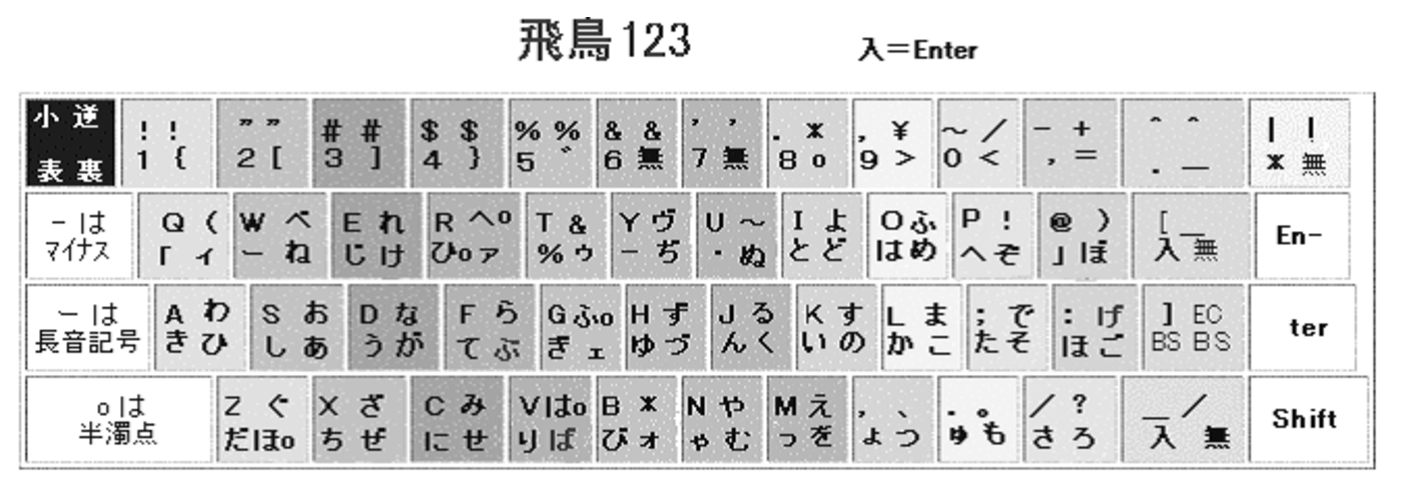
\includegraphics[width=14cm,clip]{res_tomoemon/asuka.eps}
 \end{center}
 \caption{飛鳥配列123-383版}
 \label{asuka}
\end{figure*}

\subsection{動機}

この時期に飛鳥配列を始めた理由を箇条書きにすると以下のような内容になります。
\begin{itemize}
 \item Qwertyローマ字入力の成長に限界を感じていた
 \item 日本語入力においてはローマ字入力に比べてかな入力の方が速いのは明らか
 \item JISかなは過去に取り組んだ結果4段使う特徴が自分に合わない
 \item たまたま飛鳥配列を紹介してもらった
\end{itemize}
1つ目はどちらかというと消極的な理由で、まさに本記事の「はじめに」で述べた状況にあって、わらにもすがるような気持ちで他の配列をやってみようと思いました。今振り返っても、Qwertyローマ字でもっと練習すればタイプウェルにおける最高ランクはもう少し上げることはできると思いますが、当時の時点でQwertyローマ字入力の打ちにくい部分が目についていたため、無理にその練習をする気も起きず、すっぱりとそちらの可能性は切り捨てました。

2つ目以降の理由について、かな入力と一括りに言ってもJISかなや飛鳥配列以外にも多くの配列が存在しており、当時も飛鳥配列を知る前に月配列を紹介されていたのですが、もともと親指シフトに興味を持っていたことから飛鳥配列に決めました。昔のワープロ入力コンテストでは親指シフト入力の利用者が大会を総なめにしていた、というような話をよく聞いていたことから、漠然と親指シフトはすごいという印象がありました。一方で、親指シフトについて調べてみると、シフトを行う操作を打鍵数から除いてあたかも非常に少ない打鍵数で紹介するような例が多々あり、若干うさんくさいなという印象も持っていました。
後々になって調べてみたところでは、前者については頻出単語を辞書登録のような形で登録していただけのようであり、結局タイパーが求めるような入力速度を容易に実現できるものではないこともわかっています。

このように、親指シフトを使うことで圧倒的な速度が得られるわけではないという認識が初めからあったのですが、自分の知る限りタイパーが親指シフトで限界付近まで練習した例を聞いたことがなかったので、チャレンジャーとしてやってみたいという気持ちが多分にあった配列選択だったと思います。

\subsection{練習方法}

過去の配列習得時の練習はすべて「いきなりタイプウェルを起動して打ち始める」という極めて単純な練習方法だったのですが、飛鳥配列では1つのキーに3つのかなが割り当てられており、その練習方法ではなかなかキーの位置を覚えられないと思い、一部のキーや親指シフトだけを使った単語を順番に練習していくという方法を取りました。

その際、「飛鳥のために」という単語集を教えていただき、以下のようなパターンで練習を行いました。その5,6,7と進むにつれて頻度の低い文字を含んだ単語になっていきます。
\begin{itemize}
 \item その1: シフト無しホームポジション
 \item その2: 「です」「ます」「する」等の文末と連続シフト体験
 \item その3: シフトありホームポジション
 \item その4: 右手の上下段(助詞と促音と\ruby{拗音}{ようおん}を含む)を習得する
 \item その5-7: 1~4以外のかな
 \item その8: 1ワード中にシフトの切り替えがあるもの
\end{itemize}
この練習方法は初めからすべてのかなをごっちゃに混ぜた単語の練習をするよりもかなり効率が良く、その後のAZIKの練習の際にも取り入れています。
というのも、初めて練習する配列では1文字入力するたびに毎回かなを配列図の中から探すことになります。探しては打ち、探しては打ちを何度も繰り返して少しずつ頭と体に覚え込ませていくのですが、すべてのかなを含んだ単語を練習していると配列図の中からかなの位置を探す時間が非常に長くなります。アルファベットであれば26個から探せばよいだけですが、飛鳥配列の場合は70以上のかなから探さなければなりません。
プログラミングの世界でも分割統治といって複雑な問題を分解していって、できるだけ単純な方法で解を見つけるという考え方がありますが、配列を習得する際もできるだけ練習対象の配列を分割して単純で簡単な練習になることを心がけるのが良いでしょう。


\subsection{練習結果}

最終的に2008年の段階でタイプウェル国語Kで基本常用語XS、総合XAに到達しました。最終的にと書いたのは速度面ではこれがほぼ限界で、これ以上の速度を安定して出すことは難しいと判断したからです。2011年現在でタイプウェル国語Kの基本常用語1位のランクがZDであることを考えると、足元にも及ばなかったというのが客観的な事実です。個々人の能力の差があるため、私以外のタイパーが取り組めばもっと上に行ける可能性はありますが、やはり親指シフトを使うという特性上難しいと感じました。

JISかな入力やローマ字入力と大きく違うのは、やはり親指を使ってシフトキーを他のかなキーと同時に押す操作です。配列変更ソフトの設定によっては、親指シフトを押してからかなを押す場合だけではなく、逆にかなを押してから親指シフトを押すことでシフトが必要な文字を入力できます。これはシフトを押すタイミングに許容できる誤差を含めておくということなのですが、私の経験では高速に打てるようになってくるとこの許容誤差によるミスが多発したため、「親指シフトを押してからかなを押す場合にのみシフトを有効にする」設定で練習していました。しかし、それでも入力速度が速くなればなるほど親指シフトを押すタイミングがシビアになってくるため、シフトのずれによるミスの発生が顕著になります。これは飛鳥配列に限らず親指シフト系全般に言えるのではないかと感じました。

上記の通り、飛鳥配列の取り組みは速度向上という観点から言えば失敗です。
高速入力した時の親指シフトの特徴についてある程度把握できた、配列習得の効率良い練習方法について学ぶことができたというメリットはありましたが、これで良かったと配列習得を繰り返していたはただの配列マニアになってしまいます。本気で(少なくとも短期間で)トップタイパーを目指す人にとってはこのような取り組みは避けた方が良いと断言します。自分に最も適した一つの配列にすべての練習時間を注ぎ込むことこそが、入力速度を鍛える一番の方法だからです。


\section{配列変更の例2 - tomoemon-AZIK}

\subsection{特徴}

AZIKはすでに紹介したとおり、Qwertyローマ字入力をベースにして省打鍵入力ルールを追加した配列です。tomoemon-AZIKはAZIKのルールをほぼそのまま使いつつ、さらに独自の省打鍵ルールを追加した配列になります。特に、表\ref{tomoemon:compare_roman_azik_tomoemon_azik}のように「き」「む」といったかなを入力する際に発生する同指打鍵をできるだけ避けるパターンを追加しているのが特徴です。
\begin{table*}
\begin{center}
\caption{ローマ字入力、AZIKとtomoemon-AZIKの比較}
\label{tomoemon:compare_roman_azik_tomoemon_azik}
\begin{tabular}{cccc}
\hline
かな & ローマ字入力 & AZIK & tomoemon-AZIK \\
\hline
むた むち むつ & muta muti mutu & mfta mfti mftu & mta mti mtu \\
きた きち きつ & kita kiti kitu & kfta kfti kftu & kta kti ktu \\
\hline
\end{tabular}
\end{center}
\end{table*}


\subsection{動機}

飛鳥配列の次に取り組んだ配列がAZIKで、時期的には飛鳥配列で総合XAを出した半年後に始めています。詳しい動機については私の当時の日記を見返しても書いていないので確実なことは書けないのですが、おそらく飛鳥配列の練習経験から生まれた次の二点が大きな理由だったと思います。飛鳥配列の習得までに時間がかかったので、学習コストが低そうなものに食指が動いたのが一点。もう一点は飛鳥配列は親指シフトという新たな特性によって速度の制限がかかってしまったが、既存の配列を改善して作った配列ならば従来よりも速くなるのはほぼ確実であろうということ。
このように考えると、もともとAZIKに関心を持っていたこともあり、飛鳥配列のあとにAZIKを選んだのは必然だったのかもしれません。

\subsection{練習方法}

\subsubsection*{パターン分割練習}
飛鳥配列の練習時と同様に、AZIKでも新たに追加された以下のパターンを順番に練習していく方法を取りました。

\begin{itemize}
 \item 『っ』専用キー
 \item 『シャ』『チャ』行キー、小字キー
 \item 『○ん』\ruby{撥音}{はつおん}拡張
 \item 『ァい』『ゥう』『ェい』『ォう』
 \item 『ー』長音互換キー
 \item 「Y」の代わりの「G」
 \item 「Z」の代わりの「N」
 \item 「U」「I」等の代わりの「F」
 \item 外来語の入力(外来語入力拡張)
\end{itemize}

それぞれ以下のような単語を練習しています。
\subsubsection*{パターン1:『っ』専用キー}
「っ」は\key{;}のキー単独で入力することで同指打鍵を減らします。
\begin{itemize}
 \item バッグ [ba;gu]
 \item カラット [kara;to]
\end{itemize}

\subsubsection*{パターン2:『シャ』『チャ』行キー、小字キー}
「しゃ」行は「x」、「チャ」行は「c」を子音として使い、「sha」「cha」などと比べて一打鍵減らすことができます。
\begin{itemize}
 \item しょうせい [xousei]
 \item あたしゃ [ataxa]
\end{itemize}

\subsubsection*{パターン3:『○ん』撥音拡張}
後ろに「ん」が続く文字は本来の母音キーの1つ下を使います。「もん」の場合は\key{O}の1つ下の\key{L}を使って\key{M}\key{L}と打つことで一打鍵減らすことができます。
\begin{itemize}
 \item もんだい [mldai]
 \item みんな [mkna]
\end{itemize}

\subsubsection*{パターン4:『ァい』『ゥう』『ェい』『ォう』}
高い頻度で出現する母音の連続をひとまとめにしたパターンです。「子音+ai」を「子音+q」、「子音+uu」を「子音+h」、「子音+ou」を「子音+p」といったローマ字に割り当てることで1打鍵減らします。
\begin{itemize}
 \item ごうとう [gptp]
 \item ようかい [ypkq]
\end{itemize}

上記のようなローマ字のパターンに対して、それぞれワードを数百個ずつ抽出してWeatherTypingで練習するという方法を取りました。各パターンについての練習テキストを手動で作っていくのが面倒だったので、「配列習得のtomo」というテキスト抽出フィルタソフトを作成したので、興味のある方はググってみてください。ソフト自体で辞書ファイルを持っていて、指定したパターンのワードを自動的に抽出することができます。

\subsubsection*{パターン最適化練習}
AZIK練習で難しいポイントの一つが単純に新しく追加されたルールをほいほい使っていれば良いわけではないという点です。どういうことかというと、新しく追加されたルールを使うと、逆に打ちづらくなってしまう場合があるということです。例えば「ギガバイト」という文字列を打つときは次のようになります。

\begin{itemize}
 \item AZIK: ギガバイト [gigabqto]
 \item Qwerty: ギガバイト [gigabaito]
\end{itemize}

手元で少し試してみて欲しいのですが、\key{B}から\key{Q}に小指を伸ばすのがきつく、Qwertyローマ字入力の通りに打ったほうが楽になることがわかります。もちろん、人によってはAZIKのパターンの方が打ちやすいという方もいるかもしれませんが、これまで使わないキーをローマ字入力で使うことによって、逆に指の動きがきつくなってしまうパターンというのが存在します。
どのパターンをどの場合に使って、どの場合に使わないのかを見極めるのがAZIKの練習では非常に重要になります。

私の場合は各種タイピングソフトで練習していく中でAZIKのパターン通りに打つと打ちにくくなるパターンを表\ref{tomoemon:later_azik}、表\ref{tomoemon:non_azik}のようにまとめていきました。これに関しては人によって大きく差が出るので、みんながみんなこのとおりになるわけではありません。実際、ブログに打ちにくいパターンを書いたら「せい」は「ss」の方が速いという方もいました。もし、AZIKの練習をする際はこのような自分が苦手なパターンは気づいたらまとめていき、できるだけ使わないようにするか、あるいは念入りに練習することを心がけるのが良いでしょう。

\begin{table*}
\begin{center}
\label{tomoemon:later_azik}
\caption{AZIK拡張を使うことでQwertyよりも遅くなるパターン}
\begin{tabular}{cccl}
\hline
かな & AZIK & ローマ字入力 & 補足 \\
\hline
せい & ss & sei & \\
ディスク & dcisuku & dhisuku & 後々 [dyi] で「でぃ」を打てるように変更 \\
ティー & tgi- & thi- & 後々 [tyi] で「てぃ」を打てるように変更 \\
スポンジ & suplji & suponji & 苦手語句練習をしたら結構打ちやすくなった \\
アンケート & annke-to & anke-to & 後々「@」でも「ん」を入力できるように変更 \\
XaXai: わかい等 & wakq & wakai &  \\
ぽっと & po;to & potto & 右手小指が大変 \\
\hline
\end{tabular}
\end{center}
\end{table*}

\begin{table*}
\begin{center}
\label{tomoemon:non_azik}
\caption{他に選択肢があり、基本的にどの場面でも使わない方がいいAZIK拡張}
\begin{tabular}{ccl}
\hline
かな & AZIK & 補足 \\
\hline
せい & ss & 同指打鍵になるのでseiの方が良い \\
xん: わん等 & wz & wnの方が打ちやすい \\
ばい & bq & 普通にbaiの方が楽 \\
\hline
\end{tabular}
\end{center}
\end{table*}

この点から分かる通り、AZIKは一つの文字列の打つにしてもQwertyローマ字入力に比べて多くの打ち方が存在します。初めのうちはどのパターンをどの場面で使うかを頭で一つ一つ確認して練習する必要があり、高速なタイピングを目指すならばそれを体に覚え込ませなければなりません。

\subsection{練習結果}

Qwertyローマ字入力を改善した配列なのだから、必ず速くなるだろうと甘い見通しだったのですが、実際にタイプウェルの記録を完全に塗り替えられたのは1年以上経ったあとでした。といっても、毎日みっちりと練習していたわけではなくタイプウェルをプレイした日数でいうと約90日になります。

時間がかかったのはやはり練習方法の項に書いた、どのパターンをどこで使うかを体に覚え込ませる点です。また、AZIKからtomoemon-AZIKへの大幅なパターン追加の検討といった、本来の配列練習から少し離れた箇所でも時間を要しました。配列の改造は、一度始めると自分が納得する形になるまでに時間がかかることもあって、必ずしも高速タイピングを目指す人におすすめするわけではありませんが、私の場合は結果的に非常に満足のいく配列にできたと思っています。
ここでいう満足とは当然第一に「より速く打つことができる」ことであり、さらに「打ちやすくなった」ということでもあります。これまでに習得した配列はすべてタイピングソフトで打つための配列でしかなかったのですが、tomoemon-AZIKが非常に打ちやすいこともあり、現在は仕事やブログを書くといったPCを使うすべての場面でこの配列を使用しています。
競技タイピングにおける高速化を目指す上で必ずしも実用面の打ちやすさを重視する必要はありません。なぜなら、競技タイピングは基本的にコピー打鍵で、実用面では基本的に創作打鍵という大きく異なるスタイルだからです。私自身ももともと日常における使用まで考えていたわけではないので、この結果は偶然の産物と言っていいでしょう。ただ、AZIKを導入するの上で専用ソフトが必要ないという点も各PCに導入しやすいというメリットを生んでいるのは確かです。


\section{どうやって配列を選択すべきか}

ここまで配列習得の試行錯誤について紹介してきました。これから新たに配列を習得しようと考えている人は「過去にA配列をやっていた人は配列X、B配列をやっていた人は配列Y」のような「配列選択フローチャート」を期待されていたかもしれません。たしかにそういうものがあれば便利ですが、これまで説明してきた通りどの配列も非常に複雑な特徴を持っています。新たに習得する人によってさらに新しい特徴が見つかる可能性もあります。さらに、習得しようとする人の得意な指の動きといったように人それぞれの特徴もあります。現時点でこの両者を組み合わせたフローチャートを作るのは難しいので、将来の私かこれを読んでいるあなたにお任せしたいと思います。

フローチャートは提供できませんが、これまでの経験の中からいくつか指針だけは残しておきます。

\subsection{自分の特徴を知れ}

自分のことなので自分が一番知っているはずですが、配列を選ぶ上ではそれを明確にする必要があります。就活における面談で「あなたの長所、短所は何ですか?」を聞かれるのと同じです。長所、短所で会社の求める人材とマッチしているかどうかを判断するのと同じように、配列とのマッチングを行う際にもあなたの特徴とすり合わせる必要があります。
今の配列を使っていて、普段キーボードを打っていて、何を好み、何を苦手とするかをはっきりさせてください。できるだけ苦手な要素が少なく、好みに感じる要素が多い配列を選ぶのが重要です。例えあるタイパーが高速記録を残している配列だとしても、あなたが苦手だったり嫌いな要素が多い配列ではそもそも練習する気が起きず、速くなりようがないのです。私にとってキーボード4段を使うJISかな配列がまさにそれに当てはまりました。

\subsection{配列のデメリットを知れ}

ここまでの説明を読んでもらえればわかる通り配列にはいずれもメリットとデメリットが存在します。メリットについては配列の作者や使用者が宣伝しているのでわかりやすいのですが、デメリットについては実際に経験してみないとわからないということが多々ありえます。後になってデメリットに気づいて時間を無駄にしたと感じることを避けるためにも、事前にデメリットについて十分調べ、過去の使用者が練習の中で感じたことを自分に当てはめてその配列の適性を検討してみるのが良いでしょう。例えば、自分と同じ配列を使っていた人が新たにその配列を練習して感じたデメリットは、あなた自身もデメリットに感じる可能性が高いといえます。
自分が人柱になってでも配列の特徴を調べたい、という場合を除いては必然的に情報量が少なくなる使用者の少ない配列に取り組むのはおすすめできません。


\section{これから配列を練習するあなたへ}

この記事では配列を変更して速度を向上させるという手法について説明してきました。配列そのものや配列習得過程において明らかになっていない部分も多く、あいまいな記述が多かったと私自身感じていますが、配列を変えることで以前に比べて速く打てるようになったタイパーがいることもまた事実です。もし、これを読んで配列を変えることに対して少しでも興味を持ったらぜひ、今どんな配列があってどんなタイパーが練習しているか調べてみてください。

そして、もし新たな配列をやってみようと思ったら、ぜひやっていただきたいことがあります。

\noindent \textbf{「練習方法や練習の中で感じたことをぜひブログ等に残してください。」}

\noindent デメリットを知れの項にも書きましたが、情報量が少ない配列に取り組むことがおすすめできないということは、逆に言うと配列の練習に取り組んだ記録というのは非常に貴重な情報になるということです。あなた自身の練習の記録になるだけでなく、これからその配列や似た配列に取り組む人にとって大いに参考になります。これはあなたが著名であるか否かに関係なく、また高速タイパーである必要もありません。高速タイパーの感想がすべてのタイパーにとって有意義であるかというと必ずしもそうではなく、初心者にとっては同じ初心者の意見の方がわかりやすかったりするものです。
そして、忘れないで欲しいのは、ある配列を練習して得られる経験はその時にしか経験できないということです。よく言われる例ですが、自転車に乗れる人に向かって乗れなかった時の感覚を思い出してみろと言われてもそんなことは不可能です。いったん配列を習得してしまうと配列を習得していない状態に戻ることはできません。配列を練習しているときにしか残せないことはすべて残すようにしてください。どんなささいなことでも構いません。打っていて楽しい、小指が動きすぎて疲れる、この文字を覚えるのが難しい、といった感覚的なもので十分です。

配列変更ソフトが充実し、配列についての情報も充実しつつある今、今後も多くのタイパーが配列を変えて練習を進めていくことになると思います。あなたの練習記事がこの記事を補完し、この流れがさらに広まっていくことを切に願います。

